\chapter{Results and Discussion}\label{C:results}\label{C:evaluation}

This section reports on the outcome of several experiments involving our tool on a realistic benchmark suit. These results are in regard to the time taken, number of comparisons and the types of redundant tests identified. A range of the techniques discussed in Chapter \ref{C:workdone} will be examined, as discussed in the next section. 

There are two points that need to be taken into account before reading the results. Firstly, in the significant tables below, a `+' represents that significant increase, `-' significant decrease and `=' represents no significant difference. Secondly, the graphs are displayed using a logarithm scale.
\section{Method}

This section will go through the process of how the data was retrieved, analysed and evaluated.

Firstly, the benchmarks had to be set up in such a way that the tests could be run locally. This involved retrieving the dependencies of each benchmark and setting up an build script through ant for each, in order to run the tests. After the tests had finished, the trace information was then saved to disk.The data was then run on a grid computing setup. This setup involves a large number of computers which execute the instructions given to them. Lastly, after the results had been returned, a Wilcoxon signed rank test was used to determine whether the results are significantly different or not. A Wilcoxon signed rank test is a paired difference test that compares two related samples. The significant level used is 95\%. A total of seven different property settings were run per benchmark. Each property setting was run 30 times. 
\paragraph{}
The aim of this paper is mentioned in Section \ref{C:intro}, the main two focus points is the creation of a framework to identify redundant test cases and experimenting the different techniques on realistic benchmarks. The framework allows users to identify potentially redundant test cases however, it also gives them a range of settings and variations to use. Friction may be created if no guidance is given to users of the framework in regard to what settings to use. To create this guidance, the rest of this section explores the experiments conducted.

\subsection{Experiment \rom{1} - Pipeline Length Comparison}

The motivation behind the experiment was to analyse how the different pipeline lengths impact the performance of the framework. There were two different pipeline size's tested, two and three respectively. The final pipeline stage was the same for both pipeline sizes explored. A single pipeline comparison was left out due to the amount of memory and time taken that was required for it to finish analysing.

\begin{itemize}
\item Difference between runs: Pipeline size
\end{itemize}

\subsection{Experiment \rom{2} - K Depth Comparison}

One of the abilities of the framework is to trace the K depth specified in the settings. This experiment is to determine the impact that altering the depth of K has on the performance. There are three K depth's explored, one, two and three respectively. These were chosen after consideration in regard \todo{Finish}

\begin{itemize}
\item Difference between runs: K Depth
\end{itemize}

\subsection{Experiment \rom{3} - Parameter Comparison}

The parameters of a method call is important information, this experiment explores the performance difference between the Pipeline 2 settings as used above, with the same settings and parameters used. \todo{Redo}

\begin{itemize}
\item Difference between runs: Parameters Used
\end{itemize}

\subsection{Experiment \rom{4} - Weighting Comparison}

Utilising weighting is an attempt to remove any false positives situations. The experiment attempts to identify if weighting has any potential to remove these false positives, while exploring the impact of performance.

\begin{itemize}
\item Difference between runs: Weighting Used
\end{itemize}

\subsection{Experiment \rom{5} - Weighting and Parameter Comparison}

Combining weighting and parameters is an attempt to reduce the number of false positives, and at the same time increasing the confidence of the redundant tests being redundant. 

\begin{itemize}
\item Difference between runs: Weighting and Parameters Used
\end{itemize}

\section{Environmental Methodologies}
\label{enviro}
As previously discussed in Section \ref{performanceEvalBG} there are a variety of challenges that present themselves when using Java to evaluate the performance of a particular application. These challenges are discussed throughout the section.

\subsection{Distributed Grid Computing}
 A distributed grid computing system was used to execute the data analysis. This involved utilising idle computers located around Victoria University of Wellington's School of Engineering and Computer Science. A total of 150 jobs can be executed concurrently. If a user was to log on while a process was being conducted, the application would be paused until the user left.

\subsection{Measuring Time}
One of the variables that is considered important for evaluating the performance of the tool is the time taken. In Java, this can be achieved by accessing a system method that returns the total time in milliseconds from 1970 00:00:00 UTC to the current time. This notation of time is defined as the wall clock time taken. Utilising a distributed grid system presents difficulties with using the wall time to measure the time taken. As mentioned in Section \ref{enviro} when a job is run on the grid system, there is potential for the computer the job is running on to be paused. If wall time were to be used, the time that the process is paused would also be included. To resolve this issue, the notation of CPU time was used, this is the measure of time in nanoseconds that the thread was being executed on the CPU. Secondly, if a user logs in during analysis, the RAM being used by the JVM could potentially be moved into virtual memory dependent on the amount of RAM that the user needed. Both these issues were limited by running the tests at times when users were unlikely to log in such as overnight.
\paragraph{}
When measuring the time taken to analyse, the start up cost was not taken into account. Running up to 150 jobs meant that a large number of applications would be attempting to access a single data file at a single time. This stress on the system introduces a large amount of non-deterministic behaviour. Removing the start up cost avoided this issue.

\subsection{Hardware Environment}
\subsubsection{Heap Size}

The heap is the location that the JVM uses to store objects that are produced during the execution of an application. The amount of heap that was allocated to the JVM was 6gb for every benchmark over every run and was set through the grid system by requiring at least 6gb of free RAM before running the process on that machine. This ensured that the machine's had enough free RAM.

\subsubsection{Platform}

By using a distributed grid system, the platform required had to be specified. The platform that was used was a Linux 4.0.5 64 bit system with 8gb of RAM. This was specified through the grid system such that every machine that was used to analyse the data met these requirements.

\subsection{Software Environment}
\todo{Number of VM invocations?}

A default garbage collection strategy was used. This is known as a concurrent-mark-sweep strategy which uses multiple threads to scan the heap, mark unused objects and recycle them \cite{oracle2015}. The approach allows for a high throughput but tends to use more CPU time than other strategies. This was deemed worth the trade off as memory was the bottleneck rather than CPU for the framework and increasing the throughput was more important.

\section{Benchmarks}
\label{S:bench}
Suitable benchmarks had to be found to test the different metrics on. They were located by looking at popular java framework's, Github repositories and David Pearce's personal projects. The benchmarks had to meet a criteria where they were Java based, had reasonable number of tests (40+) and were open source. Although there were over ten potential benchmarks, the ability to use them depended on their build process. If they used Maven, it was difficult to create a jar that contained the tests and often meant that the amount of effort needed to get a working benchmark was higher than the benefit from it. This eliminated several potential benchmarks and left the projects that are built with either Ant or Gradle. In Table \ref{large_test} are the large bench marks used. These involved bench marks that required more than \todo{TODO} number of comparisons. In Table \ref{small_test} are the smaller bench marks used. 
\paragraph{}
A variety of test types and sizes of the benchmarks were examined. A range of sizes were used in order to fully evaluate the framework. Although the framework and method execution details is more aimed toward larger test suites, it would be expected that they will give the same performance in relation to large test cases with the metrics and spectra's used. A range of test types were also chosen, David J Pearce's projects contain end to end tests which run through a whole module at once, while the others attempt to test units of code at a time. Having a range of test types gives a wider evaluation view and gives insight into potential situations where method details may not be accurate in identifying redundant test cases.
\paragraph{}
For the larger benchmarks that produced up to 100,000 method calls per test, they required a large amount of memory to store it while the tests were running. Without the use of a database, this limited the number of test cases that could be collected. Whiley and Ant were the benchmarks that did not have all there tests executed.  

\begin{table}[]
\centering
\caption{Large Test Suites}
\label{large_test}
\begin{tabular}{|l|l|l|l|}
\hline
{\bf Benchmark}       &  {\bf Number of Tests} & {\bf Type of tests} & {\bf Authors}   \\ \hline
Whiley - Wyc Valid         &       &    End to End      & David J Pearce          \\ \hline
Spring - Core   &       &    Unit Tests      & Community \\ \hline
Metric-x - Core &       &    Unit Tests      & Community \\ \hline
Jasm              &             &    End to End      & David J Pearce \\ \hline

\end{tabular}
\end{table}

\begin{table}[]
\centering

\label{small_test}
\caption{Small Test Suites}
\begin{tabular}{|l|l|l|l|}
\hline
{\bf Benchmark}   & {\bf Number of Tests} & {\bf Type of tests} & {\bf Authors}  \\ \hline
Ant             &       &    Unit Tests      & Community \\ \hline
Imcache &           &    End to End        & Community \\ \hline
\end{tabular}
\end{table}

\section{Experiment \rom{1} - Pipeline Length Comparison}
\label{sec:pipelineEva}
The significant table for comparing the use of pipeline of size two vs size three is shown in Table \ref{pipelinesig}. It shows that there was a mixture of results for the total time taken to analyse the data. Metrics-x, Ant, Spring and Jasm performed significantly better with a pipeline of size 3 in comparison to size two. Imcache had no significant difference and Whiley performed significantly worse with a pipeline of size three in comparison to size two. Every benchmark has no significant difference between the number of redundant tests identified, every benchmark produced the exact same number of redundant tests in both pipeline size of two and three.
\paragraph{}
A chart showing how each benchmark reacted to the change in the pipeline size is shown in Figure \ref{fig:pipelinegraph}. It shows the number of test case comparisons that the final stage of the pipeline has to conduct.

\begin{table}[h]
\centering


\begin{tabular}{|l|l|l|}
\hline
{\bf }          & {\bf Total Time} & {\bf Redundant Tests Identified} \\ \hline
{\bf Whiley}    & +                & =                           \\ \hline
{\bf Jasm}      & -                & =                           \\ \hline
{\bf Ant}       & -                & =                           \\ \hline
{\bf Spring}    & -                & =                           \\ \hline
{\bf Imcache}   & =                & =                           \\ \hline
{\bf Metrics-x} & -                & =                           \\ \hline
\end{tabular}
\caption{A table showing the significant relationship between the use of pipeline of size two with pipeline of size three for each benchmark}
\label{pipelinesig}
\end{table}

\begin{figure}[h]
\begin{center}
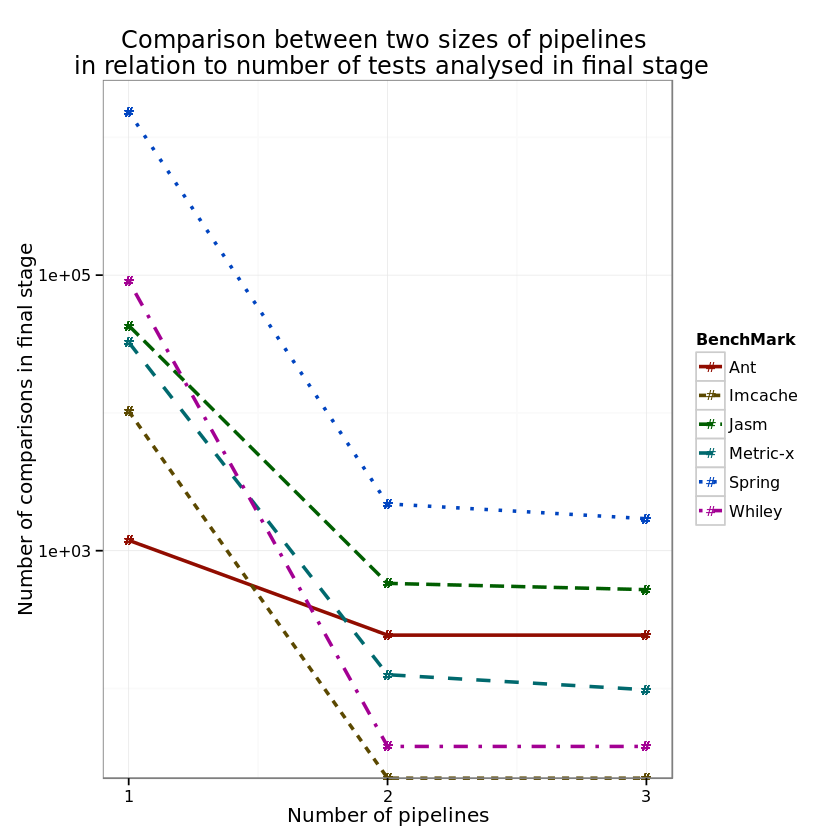
\includegraphics[height=10cm, width = 14.5cm]{Pipeline.png}
\end{center}
\caption{A figure showing the effect that using pipelines has on the number of comparisons that the final stage (Most computationally heavy) has to do.}
\label{fig:pipelinegraph}
\end{figure}



\begin{itemize}
\item Increasing the pipeline increases the performance of the framework
\item No difference between the output redundant test cases
\end{itemize}

An interesting result was the impact of the length the pipeline had on the total time taken to analyse the data. The idea of the pipeline was to decrease the amount of comparisons that the each stage in the pipeline has to do. This in turn meant less memory consumption and time taken for the more computationally heavy stages. Looking at the results show that in most cases, having two pipeline stages meant a significantly decreased total time taken to analyse over a pipeline with three stages. Intuitively, this may go against what would make sense. Looking at Figure \ref{fig:pipelinegraph}, it shows that there is a major decrease in the number of comparisons that the last stage does between one stage and two or three stages. However, between two and three stages there is limited differences. These results imply that the test cases that took less time using a two stage, were spending more time on the second stage than they were saving from the reduced number of comparisons during the third stage. 
\paragraph{}
There would be two different reasons that this result may occur. Firstly, each benchmark had it's own level of redundancy that was being looked for, this was dependent on the size of the test cases of each. As benchmarks with smaller test cases needed to have a higher level of redundancy in comparison to benchmarks with larger test cases, as this meant they would have roughly the same percentage of difference. Since each benchmark had their own percentage, this implies that each benchmark also has its optimal settings for the second pipeline. The settings were chosen by experimenting with different options. Therefore, not using a near optimal second pipeline could have contributed to it. \todo{Need to explain it better}
\paragraph{}
The second reason is that there may be little difference between the second pipeline and third pipeline. For example, if the first pipeline reduces the number of comparisons needed to 50, then there is a limited number of comparisons that a second pipeline can remove. This leads to a situation where the number of identified redundant test cases is similar for both pipelines.
\paragraph{}
As expected of the redundant tests identified, for each benchmark there was no significant change. If there were a change between the two pipelines with the same final stage settings could imply two things. Firstly, there is a bug in the code. Secondly, the second pipeline stage is more specific than the last. Since both the second stage and third stage share the same final stage, this would cause the last stage to be redundant and the redundant tests different to that of the two stage pipeline. \todo{@DJ, Does this make sense?}


\section{Experiment \rom{2} - K Depth Comparison}
Figure \ref{fig:kdepthgraph} shows the change that the KDepth had on the number of redundant test cases identified. The amount of change is limited between one, two and three depth. Ant, Whiley and Spring appear to be the most responsive. \todo{Should I do sig test?}

\begin{figure}[h]
\begin{center}
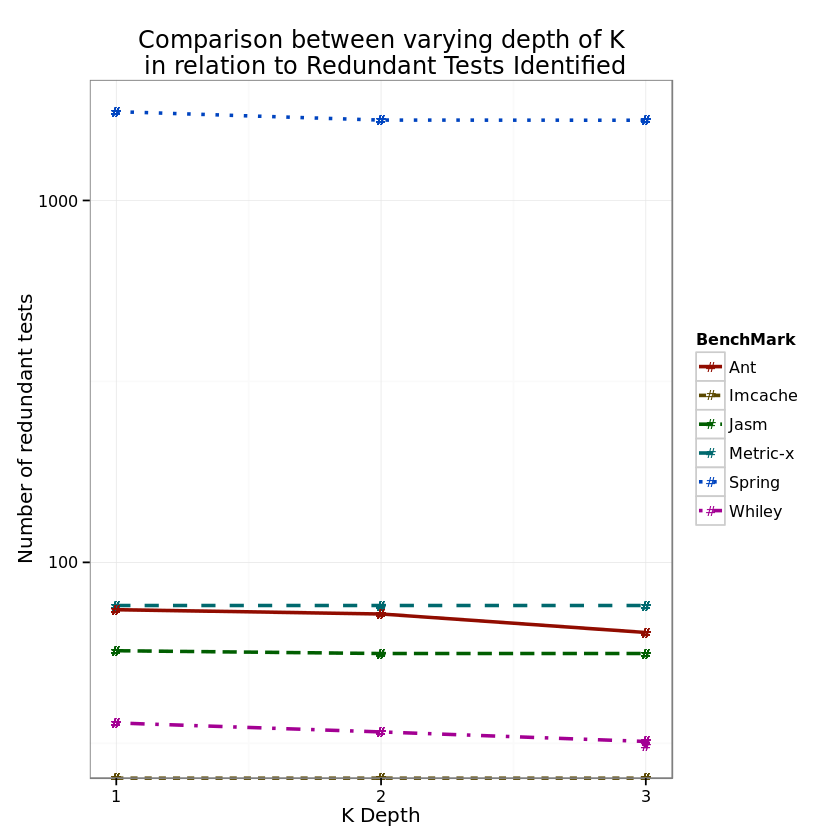
\includegraphics[height=10cm, width = 14.5cm]{KDepth.png}
\end{center}
\caption{A figure showing the effect that a change in the depth of the calling context has on the number of redundant tests are identified.}
\label{fig:kdepthgraph}
\end{figure}

\begin{itemize}
\item Increasing the K Depth has a large impact on the identified tests
\item The extra computation is worth the trade off for the increased confidence
\end{itemize}

Increasing the depth of the calling context means adding data to the analysis stages, intuitively making it more difficult for test cases to be the same. This should mean there is a decrease in the number of comparisons as the calling context depth increases. It also means that more data is going to have to be looked at which implies an increase in time as calling context depth increases.
\paragraph{}
Examining Figure \ref{fig:kdepthgraph}, it shows that the number of redundant tests is only slightly decreased as the K depth increases. This may show several things. Firstly, it may imply that when no other settings such as weighting or parameters are used, then the depth has limited effect on the redundant test cases identified. This can be seen how there is a limited amount of change for each of the benchmarks as the K increases. Secondly, the number of comparisons that were output from the first pipeline stage may cause there to be a limited differentiation. If the first pipeline stage output a low number of comparisons, then the comparisons output would more likely to be similar regardless of the K depth specified. This is due to the amount of information that the analysis stage has access to. If two test cases are practically the same method calls, except for the parameters passed to methods, then the K depth will not pick this difference up.
\paragraph{}
Overall the results imply that for some projects the calling context does not have to be particularly deep when there are no other settings used. Section \ref{sec:param} and Section \ref{sec:weight} explore the impact that using parameters has on the output.

\todo{Maybe look at a coding for the different types of tests identified. What types does lower K mean more likely to pick up ?}

\section{Experiment \rom{3} - Parameter Comparison}
\label{sec:param}

The significant table for comparing the use of parameters is shown in Table \ref{parametersig}. It shows that there was a negative relation for every benchmark in regard to time taken, this shows that parameters caused an increase in the time taken to analyse the data. Every benchmark had a significantly positive effect on the number of redundant test cases identified, showing that parameters decrease the number of redundant test cases. This is not the case in Imcache due to it having 0 redundant test cases identified in both, therefore no difference between the two.


\begin{table}[h]
\centering


\begin{tabular}{|l|l|l|}
\hline
{\bf }          & {\bf Total Time} & {\bf Redundant Tests Identified} \\ \hline
{\bf Whiley}    & +                & -                           \\ \hline
{\bf Jasm}      & +               & -                          \\ \hline
{\bf Ant}       & +                & -                           \\ \hline
{\bf Spring}    & +                & -                           \\ \hline
{\bf Imcache}   & +                & =                           \\ \hline
{\bf Metrics-x} & +                & -                           \\ \hline
\end{tabular}
\caption{A table showing the significant relationship between the use of parameters and no parameters for each benchmark}
\label{parametersig}
\end{table}

\begin{figure}[H]
\begin{center}
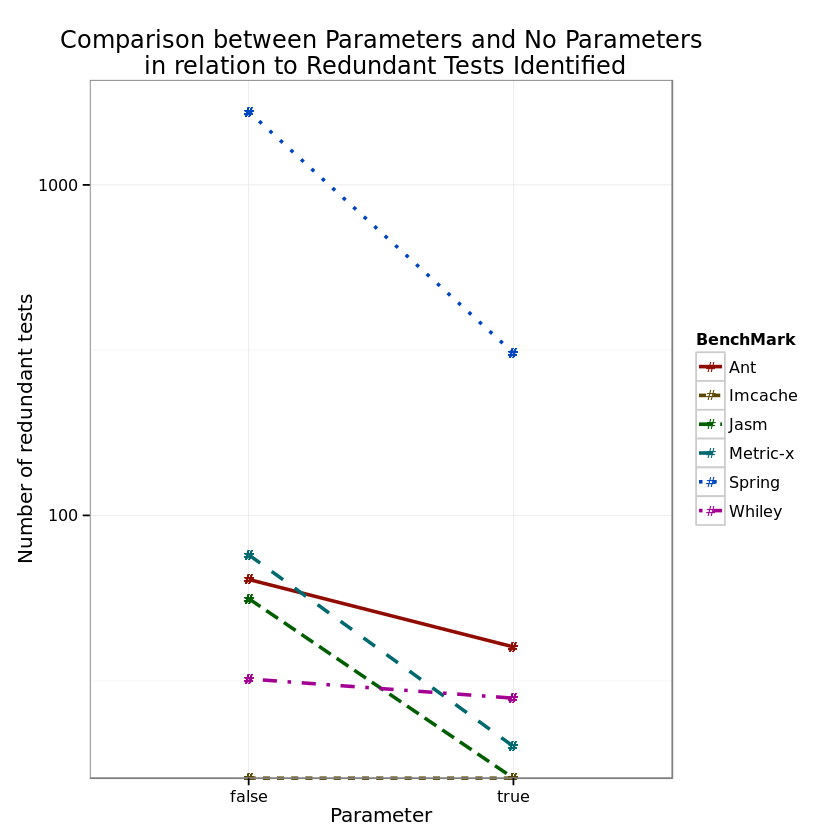
\includegraphics[height=10cm, width = 14.5cm]{Parameters.png}
\end{center}
\caption{A figure showing the effect that using parameters has on the number of redundant tests are identified.}
\label{fig:paramgraph}
\end{figure}


\begin{itemize}
\item Increases the time taken
\item Decreases the tests identified
\end{itemize}

\todo{Appears that parameters may increase the non-deterministic attirbutes of java as mentioned.}
Intuitively, recording parameters of method calls would increase the time taken to calculate the level of redundancy due to the extra amount of data generated. However, parameters only add extra computation when the method execution of the given K is exactly the same. For example, if a test execution is $A ->  B ->  C$ with D Parameter is compared to $A ->  B ->  F with E Parameter. Then the parameter won't be taken into account and therefore add limited amount o$f time. Another method which would cause time to be added is the amount of time that the VM spends garbage collecting, due to increased amount of information in memory, the garbage collection process will have to free up more memory for the analysis to continue to run.
\paragraph{}
A larger calling context would mean that it would be more difficult for two tests to match. Matching with a K value of three would be expected to be a rare occurrence in the scale of a benchmark. The parameters can be large and hold a lot of information therefore if the K value matches, then matching parameters may incur a large cost and would be expected to have limited matching. Taking into account this extra information, it would make sense that the number of redundant tests identified would decrease, but the total time taken would increase. 
\paragraph{}
Looking at the significant Table \ref{fig:paramgraph}, this matches what is expected to occur. For every benchmark, using parameters significantly increases the time taken. This may imply that the number of tests that match the K value of three was higher than expected, causing more computations to look at the parameter information. Examining Appendix \ref{fig:paramtime} shows how some benchmarks react differently to benchmarks. The most interesting would be how Jasm reacts to the use of parameters. Without parameters, it analyses the data in less than one minute, with parameters, it takes just under five minutes. One reason this may occur is the number of tests that match K value is higher than average, without weighting the set up methods are taken into account. If these set up methods are a large majority of the method calls, and match each other for the K value and parameters, this would increase the time taken substantially. Examining the weighting and parameter time taken in Appendix \ref{fig:weightparamtime}, it shows that when weighting is taken into account with parameters then for Jasm, the time taken goes from just under five minutes to just under one minute.
\paragraph{}
Every benchmark caused a significant decrease in the number of redundant test cases. This backs up the implication that there were more situations where a K depth of three matched than expected meaning that parameters had a significant effect on the redundant tests identified. Looking at Figure \ref{fig:paramgraph} shows that every benchmark reacted with a substantial decrease in redundant tests identified, with Whiley being the least affected. 

\todo{Test on Calling context = 2 ? Look at significant differences}


\section{Experiment \rom{4} - Weighting Comparison}
\label{sec:weight}
The significant table for comparing the use of weighting is shown in Table \ref{weightingsig}. There are a mix for the benchmarks in regard to the total time taken to analyse the data. Whiley, Ant and Imcache had a significantly negative relation and weighting increased the time taken to analyse. Jasm, Spring and Metric-x had a significantly positive relation and weighting decreased the time taken to analyse. Whiley, Ant, Jasm and Metrics-x had a significantly positive relation in regard to the number of redundant tests identified, showing a decrease in the number identified when weighting was applied. Spring was the only benchmark where weighting had a significantly negative impact, increasing the tests identified.

\begin{table}[h]
\centering


\begin{tabular}{|l|l|l|}
\hline
{\bf }          & {\bf Total Time} & {\bf Redundant Tests Identified} \\ \hline
{\bf Whiley}    & +                & -                           \\ \hline
{\bf Jasm}      & -                & -                           \\ \hline
{\bf Ant}       & +                & -                           \\ \hline
{\bf Spring}    & -                & +                           \\ \hline
{\bf Imcache}   & +                & =                           \\ \hline
{\bf Metrics-x} & -                & -                           \\ \hline
\end{tabular}
\caption{A table showing the significant relationship between the use of weighting and no weighting for each benchmark}
\label{weightingsig}
\end{table}


\begin{figure}[h]
\begin{center}
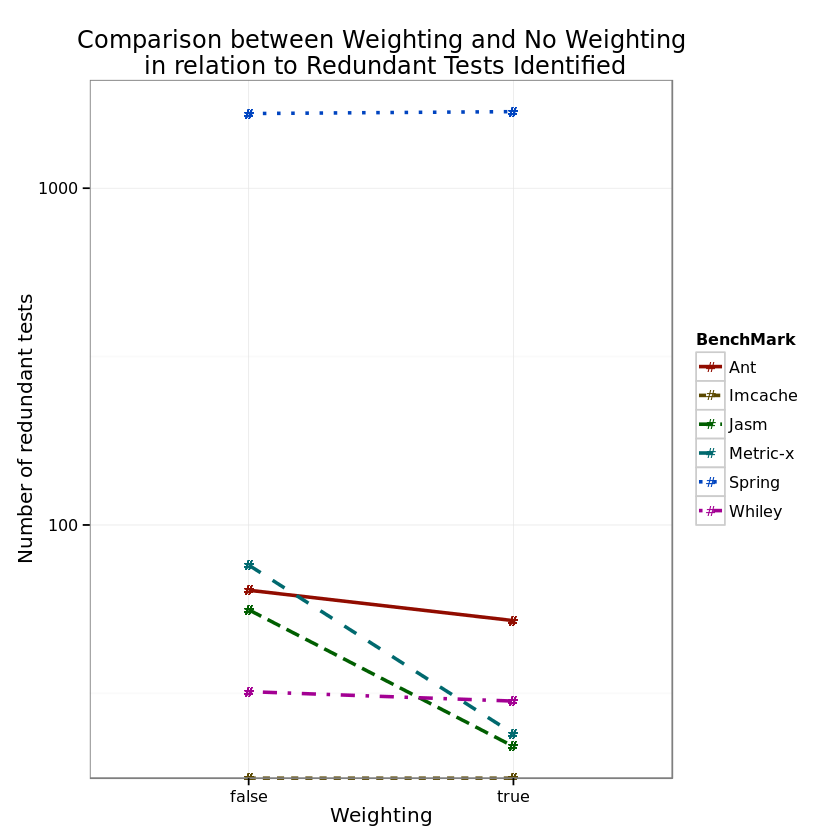
\includegraphics[height=10cm, width = 14.5cm]{Weighting.png}
\end{center}
\caption{A figure showing the effect that using weighting has on the number of redundant tests are identified.}
\label{fig:weightgraph}
\end{figure}


\begin{itemize}
\item Improves the false positive rates
\item Decreases the time taken
\end{itemize}


\todo{Weighting appears to reduce the variance in the time taken}
As previously discussed in \todo{section 2 and 3} many of the other papers encountered difficulties when test cases shared setup and teardown method calls, meaning that some of the methods picked up caused a high false - positive rate. Intuitively this makes sense when the test cases are small or the setup and teardown is large, meaning the setup and teardown methods make up a larger majority of the test calls. By taking the approach of removing a portion of the most executed method calls meant that the amount of data that would be compared decreases. This should reflect onto the results by showing a decrease in the time taken. The effect that it has on the number of redundant test cases should be dependent on the benchmark when weighting is used. This is because removing the most common tests should imply an decreased false-positive rate, but also may increase the number of actual redundant tests picked up. Therefore, depending on which on the two variables outweighs the other, will result in an increase or decrease in the number of redundant test cases identified.
\paragraph{}
Looking at the results in Table \ref{weightingsig}, it shows there was a mixture of results in regard to the total time taken. Two out of the three benchmarks that significantly increased in total time were from the small benchmarks. This may imply that the size of the benchmark has some relation to the effect of weighting on the time taken. The reason is, weighting is calculated once for each test case at the start of the pipeline stage. This weighting calculation can take a varying length of time, depending on the number of test cases. Since the weighting is linear in relation to the number of test cases, however, the comparisons is factorial in relation to the test cases. This shows that calculating the weighting for smaller benchmarks may take more time than it saves. However, the goal of weighting is not to save time, but it is to reduce the number of false positives.
\paragraph{}
Spring was the only benchmark that significantly increased the number of redundant test cases identified. The other benchmarks had a significant decrease. At first, this makes it appear that by using weighting it may solve some of the issues that were identified in \cite{koochakzadeh2009test} \cite{li2008static}. To confirm this, examining Table \ref{whileycoding} and \ref{metriccoding} will give insight into the effect of weighting. Comparing the two columns, Pipeline 2 and Weighting it shows the only difference is a removal of the two limited redundancy test cases that were picked up by Pipeline 2. The weighting is able to remove the test cases that have similar set up and tear down methods, but fails to reduce the number of other redundancies. By removing the method executions that were common throughout the benchmarks, this lead to a decrease in false-positive tests identified.


\section{Experiment \rom{5} - Weighting and Parameter Comparison}

The significant table for comparing the use of weighting with parameters is shown in Table \ref{weightingparamsig}. It shows that for every Benchmark apart from Imcache, there was a negative relation for the time taken, showing that the time increased when using weighting and parameters for the majority of benchmarks. In contrast to this, every benchmark had a positive relation to the number of redundant tests identified.

\begin{table}[h]
\centering

\begin{tabular}{|l|l|l|}
\hline
{\bf }          & {\bf Total Time} & {\bf Redundant Tests Identified} \\ \hline
{\bf Whiley}    & +                & -                           \\ \hline
{\bf Jasm}      & +                & -                           \\ \hline
{\bf Ant}       & +                & -                           \\ \hline
{\bf Spring}    & +                & -                           \\ \hline
{\bf Imcache}   & -                & =                           \\ \hline
{\bf Metrics-x} & +                & -                           \\ \hline
\end{tabular}
\caption{A table showing the significant relationship between the use of weighting with parameters and neither for each benchmark}
\label{weightingparamsig}
\end{table}

\begin{figure}[h]
\begin{center}
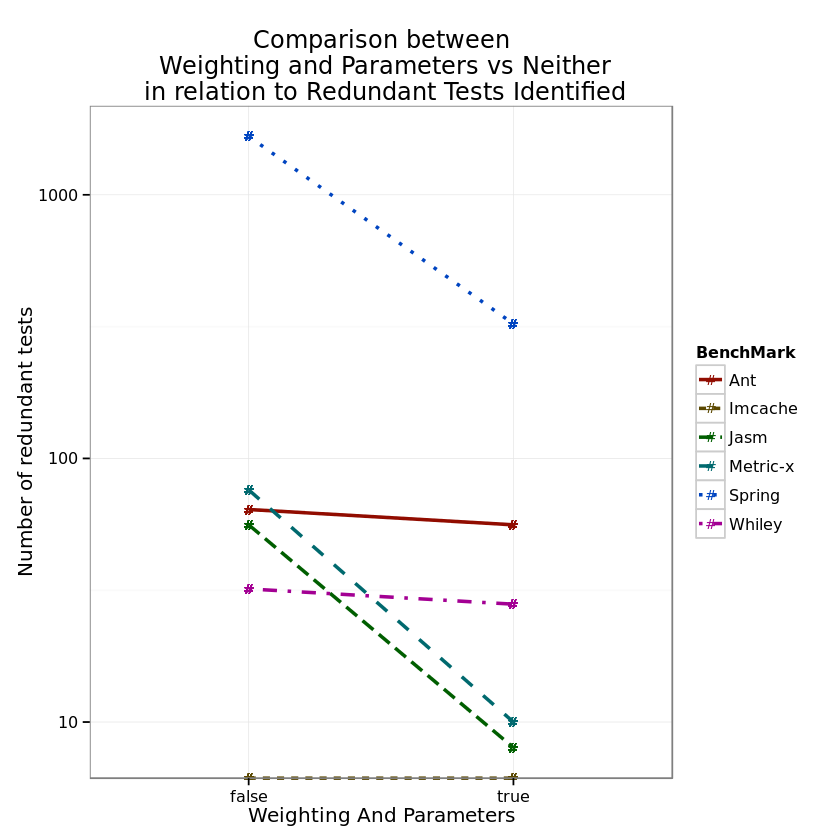
\includegraphics[height=10cm, width = 14.5cm]{WeightNParam.png}
\end{center}
\caption{A figure showing the effect that using weighting and parameters has on the number of redundant tests are identified.}
\label{fig:weightingparamgraph}
\end{figure}

\begin{itemize}
\item Improves the false positive rates
\item Decreases the time taken
\end{itemize}

\todo{More}
The result from a combination of both, weighting and parameter provides an interesting set of results. Looking at Table \ref{weightingparamsig}, it shows that it is nearly identical to the parameters table with the only exception being that the Imcache benchmark changed from significant increase in time to a significant decrease in time. This indicates that parameters may have a stronger effect on the final outcome in comparison to weighting. This is an unexpected result. As previously discussed in Section \ref{sec:param}, one of the reasons that parameters increase the time taken is due to the similar setup and tear down method calls, causing the number of k depth matches to increase and the parameters to be examined more often. With weighting removing a large portion of the common method executions it would be expected that the portion of K depth matches decreases in relation to the number of method calls, causing a decrease in time between weighting and parameters combined and parameters. Looking at Figure \ref{fig:weightparamvparamtime}, this appears to be true for Jasm, Metric-x, Spring and Imcache. However, for Whiley and Ant benchmarks the time to calculate the weighting information is taking longer than the comparisons saved. 



\section{Redundant Test Case Coding}

Table \ref{whileycoding} and Table \ref{metriccoding} compare the four major variations of techniques used to show the different types of redundancy that were picked up for the Whiley and Metric-x benchmarks respectively. The tables show a list of codings, these codings are the types of redundancy that the framework identified. It is important to note that the numbers represent matching test cases, not redundant pairings. Such that there are 5 pairs that are the same, but 10 tests that match \todo{A bit counter intuitive, might need to redo to be pairing?}.
\paragraph{}
Table \ref{whileycoding} shows that the use of weighting removed the two test cases that had no redundancy, parameters removed the same as weighting as well as the different array value test cases and parameters and weighting combined matched the parameters. Table \ref{metriccoding} \todo{describe metric coding table}

\begin{table}[h]
\centering

\begin{tabular}{|l|l|l|l|l|}
\hline
                          & \multicolumn{4}{c|}{{\bf Whiley}}                                                             \\ \hline
{\bf Types of redundancy} & \multicolumn{1}{c|}{{\bf Pipeline 2}} & {\bf Weighting} & {\bf Parameters} & {\bf Parameters and Weighting} \\ \hline
Different Equation Value  & 6                                     & 6               & 6                & 6                \\ \hline
Different Equation Sign   & 8                                     & 8               & 8                & 8                \\ \hline
Different Array Values    & 2                                     & 2               & 0                & 0                \\ \hline
Same                      & 10                                    & 10              & 10               & 10               \\ \hline
Limited Redundancy        & 2                                     & 0               & 0                & 0                \\ \hline
Rearranged Equation       & 2                                     & 2               & 2                & 2                \\ \hline
Extra if statement        & 2                                     & 2               & 2                & 2                \\ \hline
                          &                                       &                 &                  &                  \\ \hline
{\bf Total}               & 32                                    & 30              & 28               & 28               \\ \hline
\end{tabular}
\caption{A table displaying a list of coding's for the Whiley Benchmark for four of the different techniques used.}
\label{whileycoding}
\end{table}

\begin{table}[h]
\centering

\begin{tabular}{|l|l|l|l|}
\hline
                          & \multicolumn{3}{c|}{{\bf Metric-X}}                   \\ \hline
{\bf Types of redundancy} & {\bf Weighting} & {\bf Parameters} & {\bf Parameters and Weighting} \\ \hline
Different Parameter Value & 10              & 8                & 4                \\ \hline
Different Object Type     & 2               & 2                & 0                \\ \hline
Different Array Values    & 6               & 4                & 6                \\ \hline
Similar                      & 2               & 0                & 0                \\ \hline
Limited Redundancy        & 4               & 6                & 0                \\ \hline
                          &                 &                  &                  \\ \hline
{\bf Total}               & 24              & 20               & 10               \\ \hline
\end{tabular}
\caption{A table displaying a list of coding's for the Whiley Benchmark for four of the different techniques used.}
\label{metriccoding}
\end{table}